\documentclass[11pt,a4paper]{article}
\usepackage[T1]{fontenc}
\usepackage{lmodern,amsmath,amssymb,amsthm,microtype,booktabs,tikz}
\usepackage[margin=26mm]{geometry}
\usepackage[hidelinks]{hyperref}
\newtheorem{theorem}{Theorem}
\newtheorem{lemma}[theorem]{Lemma}
\newcommand{\N}{\mathrm N}
\newcommand{\Frob}{\operatorname{Frob}}
\newcommand{\Q}{\mathbb Q}
\newcommand{\Z}{\mathbb Z}
\newcommand{\OO}{\mathcal O}
\newcommand{\eps}{\varepsilon}
\newcommand{\sumgood}{\sideset{}{^{*}}\sum}
\title{Cubic root counts on rough squarefree integers\\in arithmetic progressions}
\author{AI-created mathematical note by GPT-6.2 Astra}
\date{22 November 2026}
\raggedbottom
\begin{document}
\maketitle
\begin{abstract}
For an irreducible monic integral cubic with nonsquare discriminant, give a good prime the weight equal to its number of roots minus one. Extend the weights multiplicatively to squarefree products of primes exceeding $(\log y)^2$. In an interval inside $(y,2y]$ the logarithmically weighted sum is $O_{f,\eps}(y^{1/2+\eps})$ in every reduced residue class, uniformly in the modulus. The fixed-polynomial estimate covers both signatures. For a fixed modulus the same cancellation replaces a one-sided prime test for the zeros of its dihedral twists by an upper bound on composites. We derive the uniformity by counting norm fibres on a quadratic lattice.
\end{abstract}

\section{From a polynomial to a signed count}
Let $f\in\Z[X]$ be as in the abstract and let $D=\operatorname{disc}(f)$.
A prime is good if $p\nmid D$. Write
\[
 t(p)=\#\{v\in\mathbb F_p:f(v)=0\}-1.
\]
An entirely split prime has weight $2$, an irreducible reduction has weight $-1$, and a linear times irreducible quadratic reduction has weight zero.
For $y\ge3$, $y\le u\le v\le2y$, put $z=(\log y)^2$. A star restricts to squarefree integers all of whose prime divisors are good and exceed $z$.
\begin{theorem}\label{th:main}
For every $\eps>0$, all integers $m\ge1$, and every $b$ coprime to $m$,
\[
 \left|\sumgood_{\substack{u<n\le v\\ n\equiv b\bmod m}}
       \log n\prod_{p\mid n} t(p)\right|
       \ll_{f,\eps} y^{1/2+\eps}.
\]
The same estimate holds for a prescribed cutoff $2\le z\le(\log y)^{2+o(1)}$ as $y\to\infty$, with the starting point allowed to depend on the cutoff function.
\end{theorem}

Let $E$ be the splitting field, $K=\Q(\sqrt D)$ and $\rho$ the standard two-dimensional representation of $S_3$. Its trace on $\Frob_p$ is $t(p)$ because the permutation representation of the three roots is ${\bf1}\oplus\rho$. Let $\psi$ be one of the two nontrivial characters of $\operatorname{Gal}(E/K)=C_3$, regarded by reciprocity as a finite Hecke character of $K$. Its conjugate is its inverse and $\rho=\operatorname{Ind}_{K}^{\Q}\psi$ \cite[\S3.1]{sst}. We use the incomplete ideal series
\[
 \sum_{n\ge1} A(n)n^{-s} =
 \sum_{(\mathfrak a,D)=1}\psi(\mathfrak a)(\N\mathfrak a)^{-s}.
\]
Removing a rational prime here removes all prime ideals above it. Its degree-one coefficient at a good rational prime is $t(p)$.

\newpage
\section{A quadratic norm estimate uniform in the progression}
\begin{lemma}\label{lem:uniform}
For $x\ge2$, uniformly in $m\ge1$ and $(b,m)=1$,
\[
 \left|\sum_{n\le x,\ n\equiv b\bmod m}A(n)\right|
 \ll_{f,\eps} x^{1/2+\eps}.
\]
\end{lemma}
\begin{proof}
Choose a fixed conjugation-stable finite ideal $\mathfrak f$ supported exactly above $D$, divisible by the finite conductor of $\psi$. Include both real places in the ray modulus when $K$ is real. Write $C$ for the resulting narrow ray group. For each class choose an integral ideal $\mathfrak j$ in its inverse class, prime to $\mathfrak f$. Ideals $\mathfrak a$ in the given class correspond to
\[
 \mathfrak a=(\alpha)\mathfrak j^{-1},\qquad
 \alpha\in\mathfrak j,\quad \alpha\equiv1\bmod\mathfrak f,
 \qquad |\N_{K/\Q}\alpha|\le x\N\mathfrak j,
\]
with $\alpha\ne0$, modulo congruence units. In the real case take $\alpha$ totally positive. The imaginary region is a disk, and we divide by the finite number of congruence units. In the real case choose one representative per orbit by imposing $1\le\alpha_1/\alpha_2<\eta^2$, where $\eta>1$ generates the totally positive congruence units in the first embedding. Each region is a $\sqrt{x}$ dilate of a fixed bounded region with piecewise smooth boundary. The real region has area $x\N\mathfrak j\log\eta$; the imaginary disk has area $\pi x\N\mathfrak j$ in its complex embedding. Dividing by the covolume of $\mathfrak j\mathfrak f$ gives the same leading coefficient for all classes because the factor $\N\mathfrak j$ cancels. Thus each ray class, in any \emph{fixed} narrow modulus, contains $cx+O(\sqrt x)$ such ideals. This classical estimate also follows from \cite[Theorem 1]{grs}.

For fixed $m$, project to $b$ by Dirichlet characters. The norm twist $\psi(\chi\circ\N)$ is nontrivial on the common enlarged ray group: conjugation fixes the norm pullback and interchanges $\psi$ and its distinct inverse. Summing the last class count against that twist kills the leading coefficient. Omitting ideals above $Dm$ is implemented by the enlarged ray modulus. In particular the limit of $x^{-1}\sum_{n\le x,\ n=b\bmod m}A(n)$ is zero \emph{for each} $m$.

For uniformity return to the fixed $\mathfrak f,\mathfrak j$. On $\mathfrak j$ the quadratic form $q_{\mathfrak j}(\alpha)=\N_{K/\Q}\alpha/\N\mathfrak j$ is integral. On the chosen regions it equals $\N\mathfrak a$. Partition $\mathfrak j$ modulo $m\mathfrak j\mathfrak f$. There are at most $\N\mathfrak f$ lifts per residue modulo $m\mathfrak j$. Fixing $q_{\mathfrak j}(\alpha)=b\bmod m$ yields
\[
 O_K\!\left(m\prod_{\substack{p\mid m\\p\text{ inert}}}(1+1/p)\right)
 \ll_K m\log\log(3m)
 \tag{1}
\]
residues modulo $m\mathfrak j$. Indeed $\mathfrak j$ is locally principal. Dividing by its local generator identifies $q_{\mathfrak j}$ with the local norm times a $p$-adic unit; the valuation of the norm of the generator equals that of $\N\mathfrak j$. Modulo $p^k$ every nonempty unit fibre has size the kernel size. At split and inert primes these sizes are respectively $p^k(1-1/p)$ and $p^k(1+1/p)$ by surjectivity of the norm on units in the split and unramified cases. At a ramified prime the image contains all squares of rational units, of index at most four (including $p=2$), so each fibre is $O(p^k)$. Only finitely many such primes occur. Chinese remaindering gives (1); the logarithmic bound follows from the usual maximal order of $m/\varphi(m)$.
\newpage
For each surviving coset the lattice has fixed shape and scale $m$. Its point count is area divided by covolume plus $O_f(1+\sqrt x/m)$. To see this, tile by a fixed fundamental parallelogram after division by $m$. Subdivision of each boundary arc into pieces of length at most one shows it meets $O(1+\text{length})$ tiles. Open edges and the excluded origin obey the same bound. Sum over cosets and the fixed number of ray classes with character weights. The total area coefficient vanishes by the fixed-$m$ limit proved above. This gives $O_f((\sqrt x+m)\log\log(3m))$.

There is a second bound. Since at most $k+1$ integral ideals have norm $p^k$, $|A(n)|\le d(n)$. In each divisor pair take the smaller divisor $r\le\sqrt x$. It is invertible modulo $m$; the larger divisor lies in the class $br^{-1}$. Summing $2(1+x/(rm))$ over $r$ gives $O(\sqrt x+x\log(2x)/m)$. For $m\le x$, taking the better estimate bounds the whole sum by
\[
 O_f\!\left(\sqrt{x\log(2x)\log\log(3x)}\right)
\]
because $\min(m\log\log(3x),\,x\log(2x)/m)$ is at most their geometric mean. For $m>x$ there is at most one term and $d(n)\le2\sqrt x$. This proves the lemma.
\end{proof}

\begin{figure}[ht]
\centering
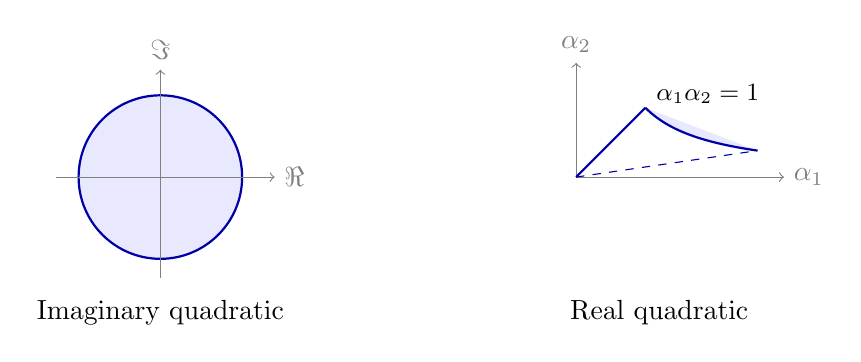
\begin{tikzpicture}[scale=.88]
\begin{scope}
\fill[blue!9] (0,0) circle (1.18);
\draw[blue!65!black,thick] (0,0) circle (1.18);
\draw[->,gray] (-1.5,0)--(1.65,0) node[right] {$\Re$};
\draw[->,gray] (0,-1.45)--(0,1.55) node[above] {$\Im$};
\node at (0,-1.95) {Imaginary quadratic};
\end{scope}
\begin{scope}[xshift=6cm]
\fill[blue!9] (0,0)--(1,1) plot[domain=1:2.618,samples=40] (\x,{1/\x})--cycle;
\draw[->,gray] (0,0)--(3,0) node[right] {$\alpha_1$};
\draw[->,gray] (0,0)--(0,1.65) node[above] {$\alpha_2$};
\draw[blue!65!black,thick] (0,0)--(1,1) plot[domain=1:2.618,samples=40] (\x,{1/\x});
\draw[blue!65!black,dashed] (0,0)--(2.618,.382);
\node[font=\small] at (1.9,1.2) {$\alpha_1\alpha_2=1$};
\node at (1.2,-1.95) {Real quadratic};
\end{scope}
\end{tikzpicture}
\caption{The regions for $\N\mathfrak a\le x$ after rescaling. Left, a disk with a finite unit action. Right, a fundamental sector for the positive unit action, drawn at normalized norm bound one with $\eta=(3+\sqrt5)/2$ in $\Q(\sqrt5)$ and trivial finite modulus. Its dashed edge is excluded. Translation of a lattice coset changes the boundary error, while the area term stays fixed.}
\end{figure}

\section{Removing small and repeated prime factors}
At a good prime the reciprocal ideal Euler factor is $1-tT+dT^2$, where $t=t(p)$ and $d=\det\rho(\Frob_p)\in\{1,-1\}$. The ratio of the desired squarefree series to the ideal series has the following factors at $p>z$:
\[
\begin{array}{c|r|r|l}
\text{cycle type}&t&d&(1+tT)(1-tT+dT^2)\\ \hline
1+1+1&2&1&1-3T^2+2T^3\\
3&-1&1&1-T^3\\
2+1&0&-1&1-T^2
\end{array}
\]
The missing linear term makes the correction absolutely summable to the right of $1/2$. At a good $p\le z$ use $1-tT+dT^2$ and at a bad prime use $1$.

\newpage
Writing $h_z$ for the coefficients of the ratio, for fixed $1/2<\sigma<1$,
\[
 \sum_{d\ge1}|h_z(d)|d^{-\sigma}
 \ll_{\sigma}\exp\{O_\sigma(z^{1-\sigma})\}.
\]
Indeed the small-prime linear terms have sum $\ll_\sigma z^{1-\sigma}$ even on summing over all integers, and the squares at large primes converge. For the stated cutoff $z^{1-\sigma}\le(\log y)^{2(1-\sigma)+o(1)}=o(\log y)$.
The required unweighted coefficients are $A*h_z$. In a reduced residue class each contributing $d$ is coprime to $m$, and the complementary factor lies in $bd^{-1}\bmod m$. Lemma~\ref{lem:uniform} gives at $y\le X\le2y$ the upper bound
\[
 X^\sigma\sum_{d\le X}|h_z(d)|d^{-\sigma}\ll_{f,\sigma}
 X^\sigma y^{o(1)} .
\]
The cutoff stays fixed while $X$ varies. Partial summation inserts $\log n$ on $(u,v]$ at cost $O(\log(2y))$. Choosing $\sigma$ sufficiently close to $1/2$ proves Theorem~\ref{th:main}.

\section{What the composite sum tests}
Fix $m$ and $\delta>0$ and take $b=1$. Write $P_m(y)$ and $C_m(y)$ for the prime and composite parts on $(y,2y]$. By Theorem~\ref{th:main}, an upper bound $C_m(y)\le c_\eps y^{1/2+\eps}$ throughout arbitrarily late windows $Y\le y\le Y^{1+\delta}$, for each $\eps>0$, is equivalent to a lower bound of that order on $P_m(y)$ on such windows.

More precisely, using the one-sided Landau-window theorem \cite{alp}, this condition is equivalent to RH for the family $L(s,\rho\otimes\chi)$, $\chi\bmod m$. To see the sign, let $J$ be their product, $-J'/J=\sum b(n)n^{-s}$ and $g(u)=-\sum_{e^u<n\le 2e^u} b(n)$. Orthogonality gives $b(p)=\varphi(m)t(p)\log p$ on good $p=1\bmod m$ and zero on the other good primes prime to $m$. Removing the finite bad primes and the powers $p^k$ with $k\ge2$ costs $O_{f,m}(\sqrt y\log^2(2y))$. For $\Re s>1$ the Laplace transform is $(2^s-1)J'(s)/(sJ(s))$. Every zero of $J$ in $\Re s>0$ gives a pole, with nonzero residue and positive residue at a real zero. The factors are entire: each comes from the nontrivial Hecke character $\psi(\chi\circ\N)$. The product has real coefficients. The window theorem applied to $g$ gives no zero with $\Re s>1/2$; the conjugate twists' functional equations give the remaining half. Conversely RH for these very factors gives the prime bound by the individual Artin-character explicit formula \cite[\S3.5]{mms} applied to their direct sum. Its trivial multiplicity is zero. Passage to logarithmic weights costs one logarithm. The formulation for the complete Dedekind zeta of a compositum must in addition account for its cyclotomic factors.

\newpage
\section{Two examples of opposite signature}
For $f_-(X)=X^3-X-1$ and $f_+(X)=X^3-4X+1$ the discriminants
are $-23$ and $229$. Both polynomials are irreducible by the rational
root test. On $8192<n\le16384$ take $b=1$, $m=5$, and
$z=(\log 8192)^2$. The cutoff includes exactly the same primes as its
integer part, $81$. In the table the counts include terms with nonzero
weight, and $P$ and $C$ denote the signed prime and composite log sums.
\begin{center}
\begin{tabular}{rrrrr}
\toprule
$D$&Primes&Composites&$P$&$C$\\
\midrule
$-23$&106&2&45.695641&$-38.245436$\\
$229$&102&2&29.017412&18.746274\\
\bottomrule
\end{tabular}
\end{center}
For an example with $m>\sqrt{2y}$, put $y=2048$, $m=131$, $b=15$ and
use the smaller cutoff $z=7$. For $f_-$ the only contributing
integers are $2111$ and $3683=29\cdot127$, of weights $-1$ and $1$.
For $f_+$ they are $2897$ and $3421=11\cdot311$, of weights $2$ and $1$.
The accompanying Python source computes these examples directly from
the roots, and also by convolution of the ideal coefficients with the
local correction factors.

\paragraph{Mathematical precedents.}
The original $X^3-269$ workshop calculation used periodic
cancellation on the Eisenstein lattice at fixed modulus. Claude
Opus 5.5 independently derived that fixed-field estimate from
Hecke coefficients. The uniform progression estimate in
Lemma~\ref{lem:uniform} counts norm fibres while keeping the quadratic
lattices fixed. A related squarefree-coefficient bound for holomorphic
newforms of even weight is due to Kowalski, Lau, Soundararajan and Wu
\cite[\S2, (2.1)]{klsw}. Their estimate makes the dependence on level
and weight explicit. Here the cubic field is fixed and the progression
modulus is arbitrary.

\small
\begin{thebibliography}{4}
\bibitem{grs} S. Gun, O. Ramar\'e and J. Sivaraman, \emph{Counting ideals in ray classes}, J. Number Theory 243 (2023), 13--37. \href{https://doi.org/10.1016/j.jnt.2022.08.005}{Theorem 1}.
\bibitem{klsw} E. Kowalski, Y.-K. Lau, K. Soundararajan and J. Wu, \emph{On modular signs}, Math. Proc. Cambridge Philos. Soc. 149 (2010), 389--411. \href{https://doi.org/10.1017/S030500411000040X}{Section 2}.
\bibitem{sst} A. Shankar, A. S\"odergren and N. Templier, \emph{Central values of zeta functions of non-Galois cubic fields}, Invent. Math. 243 (2026), 33--116. \href{https://doi.org/10.1007/s00222-025-01373-6}{Sections 3.1--3.2}.
\bibitem{mms} M. R. Murty, V. K. Murty and N. Saradha, \emph{Modular forms and the Chebotarev density theorem}, Amer. J. Math. 110 (1988), 253--281. \href{https://web.williams.edu/Mathematics/sjmiller/public_html/ntandrmt/handouts/murty/Murty_ModularFormsChebotarevDensity.pdf}{Section 3.5}.
\bibitem{alp} L. Alp\"oge, \emph{Landau window theorem}, \href{https://github.com/CocoSgt/riemann-hypothesis-lean/blob/7cbf7a0c32fca1badf05931879a37c3f8a2b03b4/src/Development/AutomorphicArithmetic/DedekindLFunctions/LandauTheorems/landauWindow.lean}{\texttt{Deduction.landau\_window}, revision 7cbf7a0}. For the fixed cubic application see the companion note \emph{A one-sided prime-interval test for all Dirichlet twists of a cubic Artin factor}.
\end{thebibliography}
\end{document}
